\documentclass{llncs}
\usepackage{latexsym}
\usepackage{times}
\usepackage{amsmath}
\usepackage{graphicx}
\usepackage{tikz}
\usepackage{pgfplots}
\usepackage{cite}
\usepackage{booktabs}
\usepackage{adjustbox}
\usepackage{marvosym}
%% Colored hyperlink 
\newcommand{\cref}[2]{\href{#1}{\color{blue}#2}}
%% Colored hyperlink showing link in TT font
% \newcommand{\chref}[1]{\href{#1}{\small\tt \color{blue}#1}}
\newcommand{\hcref}[1]{\cref{#1}{\small\tt #1}}

\bibliographystyle{splncs04}
%\bibliographystyle{abbrv}

\newcommand{\one}{\mbox{\bf 1}}
\newcommand{\zero}{\mbox{\bf 0}}
\newcommand{\leafone}{L_1}
\newcommand{\leafzero}{L_0}
\newcommand{\booland}{\land}
\newcommand{\boolor}{\lor}
\newcommand{\pand}{\mathbin{\land_{\sf v}}}
\newcommand{\por}{\mathbin{\lor_{\sf a}}}
\newcommand{\boolxor}{\oplus}
\newcommand{\boolnot}{\neg}
%\newcommand{\tautology}{\top}
%\newcommand{\nil}{\bottom}
\newcommand{\tautology}{1}
\newcommand{\nil}{0}
\newcommand{\obar}[1]{\overline{#1}}
\newcommand{\ite}{\mbox{\it ITE}}
\newcommand{\pite}{\mbox{\it ITE}_{\sf v}}
\newcommand{\oneminus}{{\sim}}

\newcommand{\opname}[1]{\mbox{\sc #1}}
\newcommand{\andop}{\opname{And}}
\newcommand{\implyop}{\opname{Imply}}

\newcommand{\turnstile}{\models}

\newcommand{\fname}[1]{\mbox{\small\sf #1}}

\newcommand{\lo}{\fname{Lo}}
\newcommand{\hi}{\fname{Hi}}
\newcommand{\var}{\fname{Var}}
\newcommand{\val}{\fname{Val}}

\newcommand{\makenode}[1]{{\mathbf #1}}
\newcommand{\nodeu}{\makenode{u}}

\newcommand{\interp}{\alpha}
\newcommand{\uinterp}{{\cal U}}
\newcommand{\interpset}[1]{{\cal M}(#1)}
\newcommand{\ring}{{\cal Z}}
\newcommand{\cost}{\sigma}
\newcommand{\density}{\rho}
\newcommand{\hashset}{{\cal H}}
\newcommand{\fhash}{h}
\newcommand{\mcount}{\mu}

\newcommand{\ifarg}{\textbf{I}}
\newcommand{\thenarg}{\textbf{T}}
\newcommand{\elsearg}{\textbf{E}}
\newcommand{\depend}{{\it D}}

\newcommand{\subs}[2]{[#2/#1]}
\newcommand{\substrue}[1]{\subs{#1}{\tautology}}
\newcommand{\subsfalse}[1]{\subs{#1}{\false}}

\newcommand{\subspace}{{\cal S}}

\title{Notes on Validated Model Counting \\ Version of \today}

\author{Randal E. Bryant}

\authorrunning{R. E. Bryant}

\titlerunning{Validated Model Counting}


\institute{
Computer Science Department \\
Carnegie Mellon University, Pittsburgh, PA, United States
}

\begin{document}

\maketitle

\section{Notation}

Let $X = \{x_1, x_2, \ldots, x_n\}$ be a set of Boolean variables.  An
{\em assignment} is a function $\interp$ assigning Boolean values to
the variables: $\interp:X \rightarrow \{\nil, \tautology\}$.  We can
also view an assignment as a set of {\em literals} $\{l_1, l_2,
\ldots, l_n\}$, where each literal $l_i$ is either $x_i$ or
$\obar{x}_i$, corresponding to the assignments $\interp(x_i)$ = 1 or 0,
respectively.  We denote the set of all assignments over these variables as $\uinterp$.

\subsection{Boolean Functions}

A {\em Boolean function} $f:2^X \rightarrow \{0,1\}$ can be
characterized by the set of assignments for which the function
evaluates to 1: $\interpset{f} = \{ \interp | f(\interp) = 1\}$.  Let
$\one$ denote the Boolean function that assigns value 1 to every
assignment, and $\zero$ denote the assignment that assigns value 0 to
every assignment.  These are characterized by the universal assignment set $\uinterp$ and the empty
assignment set $\emptyset$, respectively.


From
this we can define the {\em negation} of function $f$ as the function
$\boolnot f$ such that
$\interpset{\boolnot f} = \uinterp - \interpset{f}$.
We can also define the conjunction and disjunction operations over functions $f_1$ and $f_2$ as characterized by the sets
$\interpset{f_1 \booland f_2} = \interpset{f_1} \cap \interpset{f_2}$ and
$\interpset{f_1 \boolor f_2} = \interpset{f_1} \cup \interpset{f_2}$.

For assignment $\interp$ and a Boolean formula $\phi$ over $X$, we
use the notation $\interp\subs{x_i}{\phi}$ to denote the assignment
$\interp'$, such that $\interp'(x_j) = \interp(x_j)$ for all $j \not = i$
and $\interp'(x_i) = \interp(\phi)$, where $\interp(\phi)$ is the value obtained by evaluating formula $E$ with each variable assigned the value given by $\interp$.
In particular, the notation
$\interp(\subs{x_i}{\obar{x}_i})$
indicates the assignment in which the value
assigned to $x_i$ is negated, while others remain unchanged.

A Boolean function $f$ is said to be {\em independent} of variable
$x_i$ if every $\interp \in \interpset{f}$ has
$\interp(\subs{x_i}{\obar{x}_i}) \in \interpset{f}$.
The {\em dependency set} of $f$, denoted
$\depend(f)$ consists of all variables $x_i$ for which $f$ is {\em
  not} independent.

\subsection{Separable Cost Functions}

Let $\ring$ denote the elements of a commutative ring.  A {\em
  separable cost function} $\cost:X \rightarrow \ring$ assigns a value
from the ring to each variable.  We extend this function by defining
the cost of literal $\obar{x}_i$ as $\cost(\obar{x}_i) = 1 - \cost(x_i)$, the cost
of an assignment as
$\cost(\interp) = \prod_{l_i \in \interp} \cost(l_i)$,
and the cost of a function $f$ as
$\cost(f) = \sum_{\interp \in \interpset{f}} \cost(\interp)$.

For ring elemement $a$, we use the notation $\oneminus a$ to denote $1 - a$.

{\bf Example 1a}: Let $\ring$ be the set of rational numbers of the form $a\cdot 2^b$ where $a$ and $b$ are integers.
Let $\cost(x_i) = 1/2$ for all variables $x_i$.  The cost of every
assignment is then $1/2^{n}$, and the cost of a function is its
{\em density}, denoted $\density(f)$.  That is, the density of $f$, for which
$0 \leq \density(f) \leq 1$, 
is the fraction of assignments for which $f$
evaluates to 1, with $\density(\zero) = 0$ and $\density(\one) = 1$.  The density of a function
$f$ can be scaled by $2^n$ to compute the total number of models
$|\interpset{f}|$.  This is the core task of model counting.  Using
density as the metric, rather than the number of models, has the advantage that it does not vary when the
function is embedded in a larger domain $X' \supseteq X$.  

{\bf Example 1b}: Let $\ring$ be the set of rational numbers.  Assign a
{\em weight} $w(x_i)$ to each variable $x_i$ such that
$0 \leq w(x_i) \leq 1$
and let $\cost(x_i) = w(x_i)$.  This implements {\em weighted model counting}
under the restrictions that: 
1) the
weight of an assignment equals the product of the weights of its
literals, and 2) the weight of a variable $x_i$ and its negation
$\obar{x}_i$ sum to 1.

{\bf Example 1c}: Let $\ring$ be the set of rational numbers.  Assign
{\em weights} to each literal.  In particular, for each variable
$x_i$, define weights $w(x_i)$ and $w(\obar{x}_i)$, such that
$\beta(x_i) \doteq w(x_i) + w(\obar{x}_i) \not = 0$.  We can convert
this to the formulation of Example 1b by using weight $w'(x_i) =
w(x_i)/\beta(x_i)$ and then scaling the final result by $\prod_{1 \leq
  i \leq n} \beta(x_i)$.  Scaling eliminates the need to have the weight
of each variable and its negation sum to 1.  This form is sufficiently general
to handle the benchmarks used in weighted model counting track of the Model Counting Competition.
Using $w(x_i) = w(\obar{x}_i) = 1$ for each variable $x_i$,
gives the standard model counting of Example 1a.

{\bf Example 2}: Let $\ring$ be a finite field with $z = |\ring| \geq 2n$,
and let $\hashset$ be the set of functions
mapping elements of $X$ to elements of $\ring$.  For
two distinct functions $f_1$ and $f_2$ and a randomly chosen $\fhash
\in \hashset$, the probability that $h(f_1) \not = h(f_2)$ will be at least
$\left(1-\frac{1}{z}\right)^n \geq \left(1-\frac{1}{2n}\right)^n >  1/2$.  Therefore, these functions can be used as part of a
randomized algorithm for equivalence testing~\cite{blum:ipl:1980}.

\subsection{Computing Cost Functions}

Three key properties of separable cost functions make it possible, in
some cases, to compute the cost of a Boolean formula without
enumerating all of its satisfying solutions.


\begin{proposition}[Negation]
\label{prop:negation}
  For separable cost function $\cost$ and Boolean function $f$:
  $\cost(\neg f) = 1 - \cost(f) = \oneminus \cost(f)$.
\end{proposition}

\begin{proposition}[Variable-Partitioned Conjunction]
\label{prop:conjunction}
  For separable cost function $\cost$ and Boolean functions $f_1$ and $f_2$ such that $\depend(f_1) \cap \depend(f_2) = \emptyset$:
    $\cost(f_1 \land f_2) = \cost(f_1) \cdot \cost(f_2)$.
\end{proposition}
We use the notation $f_1 \pand f_2$ to denote the conjunction of $f_1$ and
$f_2$ under the condition that $f_1$ and $f_2$ are defined over
disjoint sets of variables.

\begin{proposition}[Assignment-Partitioned Disjunction]
\label{prop:disjunction}
  For separable cost function $\cost$ and Boolean functions $f_1$ and $f_2$ such that $\interpset{f_1} \cap \interpset{f_2} = \emptyset$:
    $\cost(f_1 \lor f_2) = \cost(f_1) + \cost(f_2)$.
\end{proposition}
We use the notation $f_1 \por f_2$ to denote the disjunction of $f_1$ and $f_2$ under the
condition that $f_1$ and $f_2$ hold for mutually exclusive assignments.




%% We also find it useful to introduce a restricted version of the
%% if-then-else operator, denoted $\pite$.  For functions $f_1$,
%% $f_2$, and $f_3$, we define $\pite(f_1, f_2, f_3) = (f_1 \pand f_2)
%% \por (\neg f_1 \pand f_3)$.  The two arguments to the disjunction are
%% guaranteed to satisfy the requirements for an assignment-partitioned
%% disjunction, since the first argument can only be satisfied by assignments
%% for which $f_1$ evaluates to $\tautology$, while the second can only
%% be satisfied by assignments for which $f_1$ evaluates to $\nil$.  The
%% only restriction of the $\pite$ operator is that
%% $\depend(f_1) \cap \depend(f_2) = \emptyset$ and
%% $\depend(f_1) \cap \depend(f_3) = \emptyset$.

\section{Separable Schemas}

Computing the cost function for a Boolean formula becomes
straightforward when the formula contains only the operations
$\pand$, $\por$, and $\neg$, as is demonstrated by
Propositions~\ref{prop:negation}--\ref{prop:disjunction}.  We define {\em separable schemas}
as a direct-acyclic graph representation of such formulas.
Representing formulas as a graph enables sharing subformulas, yielding a more compact representation.

\subsection{Schema Definition}

\begin{table}
  \caption{Recursive Definition of Separable Schemas and their Costs}
  \label{tab:schema}
%%A) Basic Operations\\
\begin{center}
\begin{tabular}{ccccc}
\toprule
  \makebox[15mm]{$S$}  & \makebox[30mm]{Restrictions} & \makebox[30mm]{$D(S)$} & \makebox[30mm]{$\interpset{S}$} & \makebox[25mm]{$\cost(S)$}\\
\midrule
  $\nil$  & None  & $\emptyset$    & $\emptyset$  & $0$\\
  $\tautology$        & None  & $\emptyset$    & $\uinterp$ & $1$ \\
$x_i$           & None  & $\{ x_i \}$    & $\{ \interp | \interp(x_i) = \tautology \}$ & $\cost(x_i)$ \\
$\neg S_1$      & None  & $\depend(S_1)$ & $\uinterp - \interpset{S_1}$ & $\oneminus\cost(S)$ \\
$S_1 \pand S_2$ & $\depend(S_1) \cap \depend(S_2) = \emptyset$ & $\depend(S_1) \cup \depend(S_2)$ & $\interpset{S_1} \cap \interpset{S_2}$
& $\cost(S_1) \cdot \cost(S_2)$\\
$S_1 \por S_2$  & $\interpset{S_1} \cap \interpset{S_2} = \emptyset$ &  $\depend(S_1) \cup \depend(S_2)$ &  $\interpset{S_1} \cup \interpset{S_2}$
& $\cost(S_1) + \cost(S_2)$\\
\bottomrule
\end{tabular}
\end{center}
%% B) Composite Operations\\
%% \begin{center}
%% \begin{tabular}{cc}
%% \toprule
%%   $S$           & Definition \\
%% \midrule
%% \makebox[30mm]{$\pite(S_1, S_2, S_3)$} & \makebox[40mm]{$[S_1 \pand S_2] \por [\neg S_1 \pand S_2]$}\\
%% \bottomrule
%% \end{tabular}
%% \end{center}
\end{table}

The set of schemas over a set of variables
$\{x_1, x_2, \ldots, x_n\}$
can be defined recursively, as is shown in Table
\ref{tab:schema}.  Each schema $S$ has an associated dependency set
$\depend(S)$ and an associated set of models $\interpset{S}$.
%% We
%% divide the operations into {\em basic} ones that are fundamental to
%% the representation, and {\em composite} ones that can be constructed
%% from basic operations.  The latter category consists of just the $\pite$ operation.
A key property of a Boolean formula represented by separable schema
$S$ is that, for any separable cost function $\cost$, the cost of the
formula $\cost(S)$ can be computed with a linear number of ring
operations, as is shown in the final column of Table~\ref{tab:schema}.

\subsection{Schema Normalization}

\begin{table}
  \caption{Normalization Rules}
  \label{tab:normalize}
  \begin{center}
  \begin{tabular}{ccccccc}
    \makebox[20mm]{$\neg \nil$} & \makebox[5mm]{$\rightarrow$} & \makebox[20mm]{$\tautology$} & \makebox[15mm]{} &
    \makebox[20mm]{$\neg \tautology$} & \makebox[5mm]{$\rightarrow$} & \makebox[20mm]{$\nil$} \\
    $\neg \neg S$ & $\rightarrow$ & $S$ \\
    $S \pand \nil$ & $\rightarrow$ & $\nil$ && $\nil \pand S$ & $\rightarrow$ & $\nil$ \\
    $S \pand \tautology$ & $\rightarrow$ & $S$ && $\tautology \pand S$ & $\rightarrow$ & $S$ \\
    $S \por \nil$ & $\rightarrow$ & $S$ && $\nil \por S$ & $\rightarrow$ & $S$ \\
    $S \por \tautology$ & $\rightarrow$ & $\tautology$ && $\tautology \por S$ & $\rightarrow$ & $\tautology$ \\
%%     $\pite(\neg S_1, S_2, S_3)$ & $\rightarrow$ & $\pite(S_1, S_3, S_2)$ \\
%%     $\pite(\tautology, S_2, S_3)$ & $\rightarrow$ & $S_2$ & &
%%     $\pite(\nil, S_2, S_3)$ & $\rightarrow$ & $S_3$ \\
%%     $\pite(S_1, \tautology, \nil)$ & $\rightarrow$ & $S_1$ &&
%%     $\pite(S_1, \nil, \tautology)$ & $\rightarrow$ & $\neg S_1$ \\
%%     $\pite(S_1, S_2, \nil)$ & $\rightarrow$ & $S_1 \pand S_2$ & &
%%     $\pite(S_1, \nil, S_3)$ & $\rightarrow$ & $\neg S_1 \pand S_3$ \\
%%     $\pite(S_1, S_2, \tautology)$ & $\rightarrow$ & $\neg [S_1 \pand \neg S_2]$ & &
%%     $\pite(S_1, \tautology, S_3)$ & $\rightarrow$ & $\neg [\neg S_1 \pand \neg S_3]$ \\
  \end{tabular}
  \end{center}
\end{table}

Table~\ref{tab:normalize} shows a list of {\em normalizing}
transformations to simplify a separable schema.  These 
eliminate extra negations and remove constant
terms, such that constants only occur in schemas when representing constant functions $\zero$ and $\one$.
%% The most interesting are the two bottom rules, which
%% use DeMorgan's Laws to simplify an $\pite$ operation when one of
%% the arguments is $\tautology$ into a $\pand$ operation.  We will make use of this
%% transformation when using BDDs to convert a set of clauses into a
%% separable schema.

\subsection{Encoding the ITE Operation}
\label{sec:ite}


The if-then-else (ITE) operation arises when converting the CNF
representation of a formula into a separable schema, both for
bottom-up approaches based on decision diagrams, and for top-down
approaches based on CDCL\@.  For functions $f_1$, $f_2$, and $f_3$, we
define
$\ite(f_1, f_2, f_3) = (f_1 \land f_2) \lor (\neg f_1 \land f_3)$.
Observe that the $\lor$ operation in this expression satisfies
the requirements for $\por$, since the first argument can only yield
$\tautology$ for assignments that yield $\tautology$ for $f_1$, while
the second can only yield $\tautology$ for assignments that yield
$\nil$ for $f_1$.  Therefore, the only condition imposed on an
expansion of $\ite$ into the allowed schema operations is that the
dependency set for $f_1$ must be disjoint from those of $f_2$ and
$f_3$.

\begin{table}
  \caption{Encodings of the ITE Operation}
  \label{tab:ite}
  \begin{center}
  \begin{tabular}{ccc}
    ITE Form & & Encoding \\
    \midrule
     $\ite(S_1, S_2, S_3)$ & $$ & $(S_1 \pand S_2) \por (\neg S_1 \land S_3)$ \\
     $\ite(\tautology, S_2, S_3)$ & $$ & $S_2$ \\
     $\ite(\nil, S_2, S_3)$ & $$ & $S_3$ \\
     $\ite(S_1, \tautology, \nil)$ & $$ & $S_1$ \\
     $\ite(S_1, \nil, \tautology)$ & $$ & $\neg S_1$ \\
     $\ite(S_1, S_2, \nil)$ & $$ & $S_1 \pand S_2$ \\
     $\ite(S_1, \nil, S_3)$ & $$ & $\neg S_1 \pand S_3$ \\
     $\ite(S_1, \tautology, S_3)$ & $$ & $\neg (\neg S_1 \pand \neg S_3)$ \\
     $\ite(S_1, S_2, \tautology)$ & $$ & $\neg (S_1 \pand \neg S_2)$ \\
  \end{tabular}
  \end{center}
\end{table}

Table~\ref{tab:ite} shows different ways to encode an ITE operation
into schema operations.  All of these require the dependency set of
the argument $S_1$ to be disjoint from those of arguments $S_2$ and
$S_3$.  The first row shows the most general case, requiring one
$\por$ and two $\pand$ operations.  The other rows show special cases,
where one or more argument is a constant.  Of these, the final two
rows are particularly noteworthy.  They make use of DeMorgan's Laws to
convert disjunctions into conjunctions.  In particular, for Boolean
functions $f_1$ and $f_2$, we can write $\ite(f_1, \tautology, f_2)$
as $f_1 \lor f_2$, and by DeMorgan's Laws as $\neg(\neg f_1 \land
\neg f_2)$.  Similarly $\ite(f_1, f_2, \tautology) = \neg f_1 \lor f_2 = \neg(f_1 \land \neg f_2)$.
These conjunctions can then be
encoded with $\pand$ operations, since their arguments will have
disjoint dependency sets.

\section{Proof Framework for Cost Functions}

The CRAT clausal proof framework provides a means to express a
checkable proof that a Boolean formula, given in conjunctive normal
form, is logically equivalent to a separable schema.  Once this
equivalence has been established, the schema can form the basis
for computations enabled by the
representation, including trusted model counting 

The CRAT format draws its inspiration from the LRAT format for Boolean formulas and the
QRAT format for
quantified Boolean formulas (QBF).  The following are its key properties:
\begin{itemize}
  \item
  In addition to explicit clause additions and deletions, the proof contains declarations of $\pand$ and $\por$ operations.
\begin{itemize}
\item 
  These declarations implicitly add extension variables and their defining clauses to the proof.
  This is the only means for generating extension variables or adding blocked clauses to the proof.
\item The checker tracks the dependency set for every input and
  extension variable.  When an extension variable is introduced based
  on the $\pand$ operation, the dependency sets of its arguments must
  be disjoint.  The resulting extension variable has a dependency set equal to the union of those of its arguments.
\item Declaring a $\por$ operation requires a sequence of clauses
  providing a RUP proof that the arguments are mutually exclusive.  This sequence can either be provided explicitly or inferred by the proof checker.
\item Boolean complement is provided implicitly by allowing the
  arguments of the $\por$ and $\pand$ operations to be literals and not just
  variables.
\end{itemize}
\item
  Clauses can also be added when they satisfy the RUP
  property, with respect to a sequence of existing clauses.  This sequence can
  be either supplied explicitly or inferred by the proof checker.
\item
  Deleting clauses requires proving that the resulting formula is not weaker.
  \begin{itemize}
    \item For an input clause or a clause declared by RUP addition, its
      deletion must be accompanied by a sequence of remaining clauses
      providing a RUP proof of the clause.  This sequence can either
      be provided explicitly or inferred by the proof checker.
    \item The clauses defining a $\pand$ or $\por$ operation are
      implicitly deleted by deleting the operation.  This can only be
      done when the only undeleted clauses containing
      references to the associated extension variable are those
      implicitly defined when the operation was declared.
      This implies that there can be no undeleted operations having
      the operation result as an argument.
  \end{itemize}
\end{itemize}

\subsection{Syntax}

\begin{table}
  \caption{CRAT Step Types.  $C$: clause identifier, $L$: literal, $V$: variable}
  \label{tab:crat:syntax}
\centering{
  \begin{tabular}{lllll}
    \multicolumn{4}{c}{Rule} & \multicolumn{1}{c}{Description} \\
    \midrule
    \makebox[5mm][l]{$C$} & \makebox[10mm][l]{\tt i}  & \makebox[15mm][l]{$L^{*}$ {\tt 0}} & \makebox[15mm][l]{}  & \makebox[20mm][l]{Input clause} \\
    $C$ & {\tt a} & $L^{*}$ {\tt 0} & $C^{+}$  {\tt 0} & Add RUP clause.  Explicit hint \\
    $C$ & {\tt a} & $L^{*}$ {\tt 0} &  {\tt * 0} & Add RUP clause.  Inferred hint \\
     & {\tt dc} & $C$             & $C^{+}$  {\tt 0} & Delete RUP clause.  Explicit hint \\
     & {\tt dc} & $C$             & {\tt * 0} & Delete RUP clause.  Inferred hint \\
    \midrule
    $C$    & {\tt p} & $V \; L \; L$    &                  & Declare $\pand$ operation \\
    $C$    & {\tt s} & $V \; L \; L$    & $C^{+}$ {\tt 0}  & Declare $\por$ operation.  Explicit hint \\ 
    $C$    & {\tt s} & $V \; L \; L$    & {\tt * 0}  & Declare $\por$ operation.  Inferred hint \\ 
%%        & {\tt ite} & $V \; L \; L\; L$    &                  & Declare $\pite$ operation \\
     & {\tt do} & $V$             &  & Delete operation. \\

  \end{tabular}
  }
\end{table}

Table~\ref{tab:crat:syntax} shows the set of proof rules for the CRAT
format.
As with other clausal proof formats, a variable is
represented by a positive integer $v$, with the first ones being input
variables and successive ones being extension variables.  Literal $l$
is represented by a signed integer, with $-v$ being the complement of
variable $v$.  Each clause is indicated by a positive integer
identifier $C$, with the first ones being the IDs of the input clauses and successive
ones being the IDs of added clauses.  Clause identifiers must be totally ordered,
such that clause $C$ can only reference clauses $C'$ such that $C' <
C$.  Clause identifiers need not be consecutive.

The first set of proof rules are similar to those in other clausal
proofs.  Our syntax optionally allows input clauses to be listed with
a rule of type {\tt i}.  Clauses can be added via RUP addition
(command {\tt a}), with the sequence of antecedent clauses (the
``hint'') either provided explicitly or to be inferred (indicated by the character `{\tt *}') by the proof
checker.  Similarly for clause deletion (command {\tt dc}).

The declaration of a $\pand$ operation has the form:
\begin{center}
\begin{tabular}{ccccc}
  \makebox[5mm]{$i$} & \makebox[5mm]{{\tt p}} & \makebox[5mm]{$v$} & \makebox[5mm]{$l_1$} & \makebox[5mm]{$l_2$} \\
\end{tabular}
\end{center}
where $i$ is a new clause ID, $v$ is a positive integer that does not
correspond to any previous variable, and $l_1$ and $l_2$ are signed
integers representing literals of existing variables.
This declaration implicitly causes three clauses to be added to the proof:
\begin{center}
\begin{tabular}{cccc}
\makebox[10mm]{ID} & \multicolumn{3}{c}{Clause} \\
  $i$ & $v$ & $-l_1$ & $-l_2$ \\
  $i\!+\!1$ & $-v$ & $l_1$ & \\
  $i\!+\!2$ & $-v$ & $l_2$ & \\
\end{tabular}
\end{center}
The dependency sets for the arguments represented by literals $l_1$ and $l_2$ must be disjoint.

The declaration of a $\por$ operation has the form:
\begin{center}
\begin{tabular}{ccccccc}
  \makebox[5mm]{$i$} & \makebox[5mm]{{\tt s}} & \makebox[5mm]{$v$} & \makebox[5mm]{$l_1$} & \makebox[5mm]{$l_2$} 
\makebox[5mm]{$H$} & \makebox[5mm]{$\texttt{0}$} \\
\end{tabular}
\end{center}
where $i$ is a new clause ID, $v$ is a positive integer that does
not correspond to any previous variable, and $l_1$ and $l_2$ are
signed integers representing literals of existing variables.  Hint $H$
can consist either of the single character \texttt{*}, or it can be a
sequence of clause IDs.
This declaration implicitly causes three clauses to be added to the proof:
\begin{center}
\begin{tabular}{cccc}
\makebox[10mm]{ID} & \multicolumn{3}{c}{Clause} \\
  $i$ & $-v$ & $l_1$ & $l_2$ \\
  $i\!+\!1$ & $v$ & $-l_1$ \\
  $i\!+\!2$ & $v$ & $-l_2$ \\
\end{tabular}
\end{center}
The explicit or implied hints must provide a RUP proof of the clause $-l_1 \lor -l_2$.

Finally, operator deletion ({\tt do}) specifies which operator to
delete via the extension variable associated with the operator.  Doing
so for operator $v$ requires that there is no
(undeleted) RUP clause containing a literal of $v$.
Implicitly, that means
that there is no (undeleted) operator $u$
having a literal of $v$ as one of its inputs.  The defining clauses for the operation are also deleted.

\subsection{Semantics}

A CRAT proof follows the same general form as a QRAT dual
proof~\cite{bryant:cade:2021}---one that ensures that each clause
addition and each clause deletion preserves equivalence.  With CRAT,
however, clauses are defined both explicitly and implicitly.  Starting
with the set of input clauses, the proof consists of a sequence of steps that
both add and delete clauses.  Each addition must be truth preserving
and each deletion must be falsehood preserving.  At the end, all input
clauses must have been deleted, and among the remaining clauses there
must be only a single unit clause consisting of some variable or its
complement.  Except for trivial cases, the final literal will be an
extension variable or its complement.  That literal will indicate the
root of the schema as the (possibly negated) output of a schema
operation.  Working from that root backward, the schema can be
extracted from the CRAT file.

\subsection{Example 1}

\begin{figure}
  \centering{
    \begin{minipage}{0.4\textwidth}
      A) Schema   \\[2ex]
    \centering{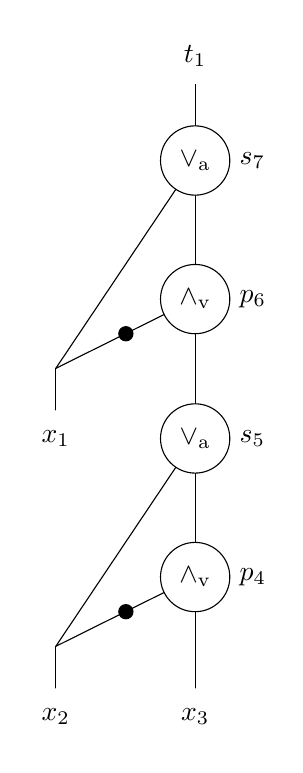
\begin{tikzpicture}
\definecolor{fillcolor}{RGB}{255,255,255}
\definecolor{highcolor}{RGB}{0,0,0}
\definecolor{lowcolor}{RGB}{0,0,0}
\definecolor{neutralcolor}{RGB}{0,0,0}
\definecolor{pathcolor}{RGB}{0,0,0}
\definecolor{background}{RGB}{225,225,225}
\draw (2.12,8.74) [thin,neutralcolor] -- (2.12,7.41);
\draw (2.12,7.41) [thin,neutralcolor] -- (0.35,4.77);
\draw (2.12,7.41) [thin,neutralcolor] -- (2.12,5.65);
\draw (2.12,5.65) [thin,neutralcolor] -- (0.35,4.77);
\draw [fill=neutralcolor,draw=neutralcolor] (1.24,5.21) circle [radius=0.09];
\draw (2.12,5.65) [thin,neutralcolor] -- (2.12,3.88);
\draw (2.12,3.88) [thin,neutralcolor] -- (0.35,1.24);
\draw (2.12,3.88) [thin,neutralcolor] -- (2.12,2.12);
\draw (2.12,2.12) [thin,neutralcolor] -- (0.35,1.24);
\draw [fill=neutralcolor,draw=neutralcolor] (1.24,1.68) circle [radius=0.09];
\draw (2.12,2.12) [thin,neutralcolor] -- (2.12,0.35);
\draw (0.35,4.77) [thin,neutralcolor] -- (0.35,3.88);
\draw (0.35,1.24) [thin,neutralcolor] -- (0.35,0.35);
\draw [thin,fill=fillcolor,draw=fillcolor] (2.12,8.74) circle [radius=0.35];
\node at (2.12,8.74) {$t_1$};
\draw [thin,fill=fillcolor,draw=neutralcolor] (2.12,7.41) circle [radius=0.44];
\node at (2.12,7.41) {$\mathbin{\lor_{\textrm{a}}}$};
\draw [thin,fill=fillcolor,draw=neutralcolor] (2.12,5.65) circle [radius=0.44];
\node at (2.12,5.65) {$\mathbin{\land_{\textrm{v}}}$};
\draw [thin,fill=fillcolor,draw=neutralcolor] (2.12,3.88) circle [radius=0.44];
\node at (2.12,3.88) {$\mathbin{\lor_{\textrm{a}}}$};
\draw [thin,fill=fillcolor,draw=neutralcolor] (2.12,2.12) circle [radius=0.44];
\node at (2.12,2.12) {$\mathbin{\land_{\textrm{v}}}$};
\draw [thin,fill=neutralcolor,draw=neutralcolor] (0.35,4.77) circle [radius=0.00];
\node at (0.35,4.77) {};
\draw [thin,fill=fillcolor,draw=fillcolor] (0.35,3.88) circle [radius=0.35];
\node at (0.35,3.88) {$x_1$};
\draw [thin,fill=neutralcolor,draw=neutralcolor] (0.35,1.24) circle [radius=0.00];
\node at (0.35,1.24) {};
\draw [thin,fill=fillcolor,draw=fillcolor] (0.35,0.35) circle [radius=0.35];
\node at (0.35,0.35) {$x_2$};
\draw [thin,fill=fillcolor,draw=fillcolor] (2.12,0.35) circle [radius=0.35];
\node at (2.12,0.35) {$x_3$};
\node [right] at (2.56,7.41) {$s_7$};
\node [right] at (2.56,5.65) {$p_6$};
\node [right] at (2.56,3.88) {$s_5$};
\node [right] at (2.56,2.12) {$p_4$};
\end{tikzpicture}%%
}
    \end{minipage}
    \begin{minipage}{0.4\textwidth}
    B) Cost Computation\\[2ex]
    \centering{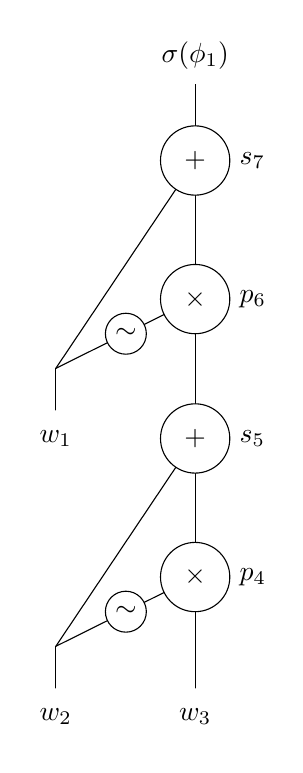
\begin{tikzpicture}
\definecolor{fillcolor}{RGB}{255,255,255}
\definecolor{highcolor}{RGB}{0,0,0}
\definecolor{lowcolor}{RGB}{0,0,0}
\definecolor{neutralcolor}{RGB}{0,0,0}
\definecolor{pathcolor}{RGB}{0,0,0}
\definecolor{background}{RGB}{225,225,225}
\draw (2.12,8.74) [thin,neutralcolor] -- (2.12,7.41);
\draw (2.12,7.41) [thin,neutralcolor] -- (0.35,4.77);
\draw (2.12,7.41) [thin,neutralcolor] -- (2.12,5.65);
\draw (2.12,5.65) [thin,neutralcolor] -- (0.35,4.77);
\draw [fill=neutralcolor,draw=neutralcolor] (1.24,5.21) circle [radius=0.09];
\draw (2.12,5.65) [thin,neutralcolor] -- (2.12,3.88);
\draw (2.12,3.88) [thin,neutralcolor] -- (0.35,1.24);
\draw (2.12,3.88) [thin,neutralcolor] -- (2.12,2.12);
\draw (2.12,2.12) [thin,neutralcolor] -- (0.35,1.24);
\draw [fill=neutralcolor,draw=neutralcolor] (1.24,1.68) circle [radius=0.09];
\draw (2.12,2.12) [thin,neutralcolor] -- (2.12,0.35);
\draw (0.35,4.77) [thin,neutralcolor] -- (0.35,3.88);
\draw (0.35,1.24) [thin,neutralcolor] -- (0.35,0.35);
\draw [thin,fill=fillcolor,draw=fillcolor] (2.12,8.74) circle [radius=0.35];
\node at (2.12,8.74) {$\sigma(\phi_1)$};
\draw [thin,fill=fillcolor,draw=neutralcolor] (2.12,7.41) circle [radius=0.44];
\node at (2.12,7.41) {$+$};
\draw [thin,fill=fillcolor,draw=neutralcolor] (2.12,5.65) circle [radius=0.44];
\node at (2.12,5.65) {$\times$};
\draw [thin,fill=fillcolor,draw=neutralcolor] (2.12,3.88) circle [radius=0.44];
\node at (2.12,3.88) {$+$};
\draw [thin,fill=fillcolor,draw=neutralcolor] (2.12,2.12) circle [radius=0.44];
\node at (2.12,2.12) {$\times$};
\draw [thin,fill=neutralcolor,draw=neutralcolor] (0.35,4.77) circle [radius=0.00];
\node at (0.35,4.77) {};
\draw [thin,fill=fillcolor,draw=fillcolor] (0.35,3.88) circle [radius=0.35];
\node at (0.35,3.88) {$w_1$};
\draw [thin,fill=neutralcolor,draw=neutralcolor] (0.35,1.24) circle [radius=0.00];
\node at (0.35,1.24) {};
\draw [thin,fill=fillcolor,draw=fillcolor] (0.35,0.35) circle [radius=0.35];
\node at (0.35,0.35) {$w_2$};
\draw [thin,fill=fillcolor,draw=fillcolor] (2.12,0.35) circle [radius=0.35];
\node at (2.12,0.35) {$w_3$};
\draw [thin,fill=fillcolor,draw=neutralcolor] (1.24,5.21) circle [radius=0.26];
\node at (1.24,5.21) {$\sim$};
\draw [thin,fill=fillcolor,draw=neutralcolor] (1.24,1.68) circle [radius=0.26];
\node at (1.24,1.68) {$\sim$};
\node [right] at (2.56,7.41) {$s_7$};
\node [right] at (2.56,5.65) {$p_6$};
\node [right] at (2.56,3.88) {$s_5$};
\node [right] at (2.56,2.12) {$p_4$};
\end{tikzpicture}%%
}
    \end{minipage}
  }
\caption{Schema \#1 for Formula $\phi_1 = x_1 \lor x_2 \lor x_3$ and its Cost Computation}
\label{fig:c3:schema}
\end{figure}

\begin{figure}
  A).  CRAT File Contents
  \begin{center}
  \begin{tabular}{lcllll}
    \multicolumn{4}{c}{File line} & & \multicolumn{1}{c}{Explanation} \\
\midrule
    \makebox[5mm][l]{\tt 1} & \makebox[7mm]{\tt i}   & \makebox[20mm][l]{\tt 1 2 3 0}   &  \makebox[30mm]{}          & \makebox[5mm]{} & \makebox[40mm][l]{Input clause}\\
    {\tt 2}        & {\tt p}   & {\tt 4 -2 3}  &            & & Declare $p_4 = \obar{x}_2 \pand x_3$ \\
    {\tt 5}        & {\tt s}   & {\tt 5 2 4}   & {\tt 3 0}  & & Declare $s_5 = x_2 \por p_4$ \\
    {\tt 8}        & {\tt p}   & {\tt 6 -1 5}  &            & & Declare $p_6 = \obar{x}_1 \pand s_5$ \\
    {\tt 11}         & {\tt s}   & {\tt 7 1 6}   & {\tt 9 0}  & & Declare $s_7 = x_1 \por p_6$ \\
    {\tt 14} & {\tt a}  & {\tt 7 0} & {\tt 13 12 8 7 6 2 1 0} & & Assert unit clause $[s_7]$ \\
             & {\tt dc}  & {\tt 1}  & {\tt 4 5 10 11 14 0} & & Delete input clause \\
  \end{tabular}
  \end{center}
B). Proof Clauses
    \begin{center}
  \begin{tabular}{lcllll}
    \multicolumn{4}{c}{Clause} & & \multicolumn{1}{c}{Explanation} \\
\midrule
    \makebox[5mm][l]{\tt 1} & \makebox[7mm]{}   & \makebox[20mm][l]{\tt 1 2 3 0}   &  \makebox[30mm]{}          & \makebox[5mm]{} & \makebox[40mm][l]{Input clause}\\
    {\tt 2} &     & {\tt 4  2 -3 0}  &     & & Defining clauses for $p_4$ \\ 
    {\tt 3} &     & {\tt -4 -2 0}    & & & \\ %%Defining clause for $p_4$ \\ 
    {\tt 4} &     & {\tt -4 3 0}    &  & & \\ %%Defining clause for $p_4$ \\ 
            &     & {\tt -2 -4 0}   & {\tt 3 0}  & &  Mutual exclusion proof for $s_5$ \\
    {\tt 5} &     & {\tt -5 2 4 0}  &     & & Defining clauses for $s_5$ \\ 
    {\tt 6} &     & {\tt  5 -2 0}    &  &  \\  %%Defining clause for $s_5$ \\ 
    {\tt 7} &     & {\tt  5 -4 0}    &  & &  \\  %%Defining clause for $s_5$ \\ 
    {\tt 8} &     & {\tt 6  1 -5 0}  &    & & Defining clauses for $p_6$ \\ 
    {\tt 9} &     & {\tt -6 -1 0}    &  & &  \\  %%Defining clause for $p_6$ \\ 
    {\tt 10} &     & {\tt -6 5 0}    &  & &  \\  %%Defining clause for $p_6$ \\ 
            &     & {\tt -1 -6 0}   & {\tt 9 0}  & &  Mutual exclusion proof for $s_7$ \\
    {\tt 11} &     & {\tt -7 1 6 0}  &  & & Defining clauses for $s_7$ \\ 
    {\tt 12} &     & {\tt  7 -1 0}     & &  \\  %%Defining clause for $s_7$ \\ 
    {\tt 13} &     & {\tt  7 -6 0}     & &  \\  %%Defining clause for $s_7$ \\ 
    {\tt 14} &     & {\tt 7 0} & {\tt 13 12 7 6 2 1 0} & & Assert unit clause $[s_7]$ \\
             & {\tt dc}  & {\tt 1}  & {\tt 4 5 10 11 14 0} & & Delete input clause \\
  \end{tabular}
  \end{center}
  \caption{CRAT file \#1 for formula $x_1 \lor x_2 \lor x_3$, and the resulting set of proof clauses}
  \label{fig:c3:crat}
\end{figure}
    
As an illustration, consider the Boolean formula
$\phi_1 = x_1 \lor x_2 \lor x_3$,
represented by a single clause.  We cannot directly use the
$\por$ operation to form these disjunctions, since the sets of assignments
satisfying the individual literals are not disjoint.  Instead, we must
decompose this formula into a sequence of operations.
Figure~\ref{fig:c3:schema}A shows one such decomposition.
The subscripts of the variables and the operator labels correspond to
the numbers of the input and extension variables in the CRAT proof.
Edges marked with dots indicate Boolean negation.

The conjunction of $\obar{x}_2$ and $x_3$ can be computed as $p_4 =
\obar{x}_2 \pand x_3$, since the literals have disjoint dependency
sets. We can then express the disjunction $x_2 \lor x_3$ as
as $s_5 = x_2 \por p_4$.  A similar process forms the
disjunction $x_1 \lor x_2 \lor x_3$ by first forming the product $p_6
= \obar{x}_1 \pand s_5$ and the final sum $s_7 = x_1 \por p_6$.

The logical representation can readily be converted into a formula for
computing $\cost(\phi_1)$, the cost of formula $\phi_1$, given a weight
$w_i$ for each variable $x_i$ for $1 \leq i \leq 3$.  This is
illustrated in Figure~\ref{fig:c3:schema}B\@.  Note how the Boolean
negations become $\oneminus$ operations.  This formula is valid for
any cost function.

Figure~\ref{fig:c3:crat}A shows an annotated version of the CRAT file
for this example, while \ref{fig:c3:crat}B shows the sequence of clauses that constitute the proof, including those defined implicitly, and those required for mutual exclusion checks.
   Clause 1
is the input clause.
Clauses 2--13 are added explcitly as the defining clauses for the four operations.
Also shown are the required mutual exclusion proofs for the two sum operations.
Proof clause 14 adds the unit clause for the extension variable $s_7$.
We refer to the literal representing formula $\phi_1$ as $t_1$,
and we therefore have $t_1 = s_7$.
The unit clause indicates that extension variable $s_7$ will evaluate to
$\tautology$  for any assigment that satisfies the formula.  We
can write this as $\phi_1 \turnstile t_1$.  The
deletion step at the end turns this around, showing that
$t_1 \turnstile \phi_1$,
and therefore the input clause can be deleted, This
completes a proof that $t_1$ is logically
equivalent to the input formula.

\subsection{Example 2A}

\begin{figure}
  \centering{
    \begin{minipage}{0.4\textwidth}
      A) Schema   \\[2ex]
    \centering{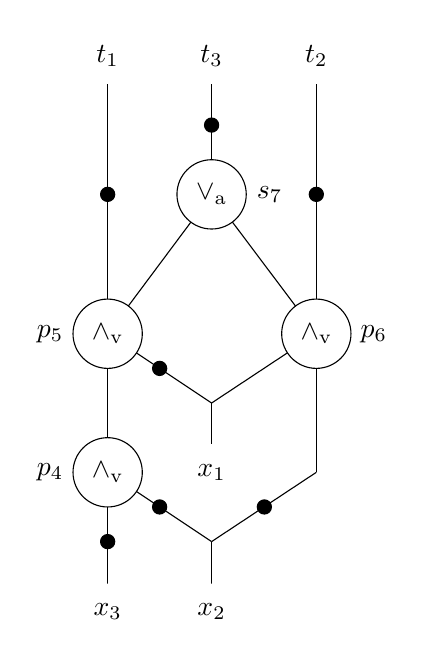
\begin{tikzpicture}
\definecolor{fillcolor}{RGB}{255,255,255}
\definecolor{highcolor}{RGB}{0,0,0}
\definecolor{lowcolor}{RGB}{0,0,0}
\definecolor{neutralcolor}{RGB}{0,0,0}
\definecolor{pathcolor}{RGB}{0,0,0}
\definecolor{background}{RGB}{225,225,225}
\draw (0.44,7.41) [thin,neutralcolor] -- (0.44,3.88);
\draw [fill=neutralcolor,draw=neutralcolor] (0.44,5.65) circle [radius=0.09];
\draw (1.76,7.41) [thin,neutralcolor] -- (1.76,5.65);
\draw [fill=neutralcolor,draw=neutralcolor] (1.76,6.53) circle [radius=0.09];
\draw (3.09,7.41) [thin,neutralcolor] -- (3.09,3.88);
\draw [fill=neutralcolor,draw=neutralcolor] (3.09,5.65) circle [radius=0.09];
\draw (1.76,5.65) [thin,neutralcolor] -- (0.44,3.88);
\draw (1.76,5.65) [thin,neutralcolor] -- (3.09,3.88);
\draw (0.44,3.88) [thin,neutralcolor] -- (1.76,3.00);
\draw [fill=neutralcolor,draw=neutralcolor] (1.10,3.44) circle [radius=0.09];
\draw (0.44,3.88) [thin,neutralcolor] -- (0.44,2.12);
\draw (3.09,3.88) [thin,neutralcolor] -- (1.76,3.00);
\draw (3.09,3.88) [thin,neutralcolor] -- (3.09,2.12);
\draw (1.76,3.00) [thin,neutralcolor] -- (1.76,2.12);
\draw (0.44,2.12) [thin,neutralcolor] -- (0.44,0.35);
\draw [fill=neutralcolor,draw=neutralcolor] (0.44,1.24) circle [radius=0.09];
\draw (0.44,2.12) [thin,neutralcolor] -- (1.76,1.24);
\draw [fill=neutralcolor,draw=neutralcolor] (1.10,1.68) circle [radius=0.09];
\draw (3.09,2.12) [thin,neutralcolor] -- (1.76,1.24);
\draw [fill=neutralcolor,draw=neutralcolor] (2.43,1.68) circle [radius=0.09];
\draw (1.76,1.24) [thin,neutralcolor] -- (1.76,0.35);
\draw [thin,fill=fillcolor,draw=fillcolor] (0.44,7.41) circle [radius=0.35];
\node at (0.44,7.41) {$t_1$};
\draw [thin,fill=fillcolor,draw=fillcolor] (3.09,7.41) circle [radius=0.35];
\node at (3.09,7.41) {$t_2$};
\draw [thin,fill=fillcolor,draw=fillcolor] (1.76,7.41) circle [radius=0.35];
\node at (1.76,7.41) {$t_3$};
\draw [thin,fill=fillcolor,draw=neutralcolor] (1.76,5.65) circle [radius=0.44];
\node at (1.76,5.65) {$\lor_{\textrm{a}}$};
\draw [thin,fill=fillcolor,draw=neutralcolor] (0.44,3.88) circle [radius=0.44];
\node at (0.44,3.88) {$\land_{\textrm{v}}$};
\draw [thin,fill=fillcolor,draw=neutralcolor] (3.09,3.88) circle [radius=0.44];
\node at (3.09,3.88) {$\land_{\textrm{v}}$};
\draw [thin,fill=fillcolor,draw=neutralcolor] (0.44,2.12) circle [radius=0.44];
\node at (0.44,2.12) {$\land_{\textrm{v}}$};
\draw [thin,fill=neutralcolor,draw=neutralcolor] (1.76,3.00) circle [radius=0.00];
\node at (1.76,3.00) {};
\draw [thin,fill=neutralcolor,draw=neutralcolor] (1.76,1.24) circle [radius=0.00];
\node at (1.76,1.24) {};
\draw [thin,fill=neutralcolor,draw=neutralcolor] (3.09,2.12) circle [radius=0.00];
\node at (3.09,2.12) {};
\draw [thin,fill=fillcolor,draw=fillcolor] (1.76,2.12) circle [radius=0.35];
\node at (1.76,2.12) {$x_1$};
\draw [thin,fill=fillcolor,draw=fillcolor] (1.76,0.35) circle [radius=0.35];
\node at (1.76,0.35) {$x_2$};
\draw [thin,fill=fillcolor,draw=fillcolor] (0.44,0.35) circle [radius=0.35];
\node at (0.44,0.35) {$x_3$};
\node [right] at (2.21,5.65) {$s_7$};
\node [right] at (3.53,3.88) {$p_6$};
\node [left] at (0.00,3.88) {$p_5$};
\node [left] at (0.00,2.12) {$p_4$};
\end{tikzpicture}%%
}
    \end{minipage}
    \begin{minipage}{0.4\textwidth}
    B) Cost Computation\\[2ex]
    \centering{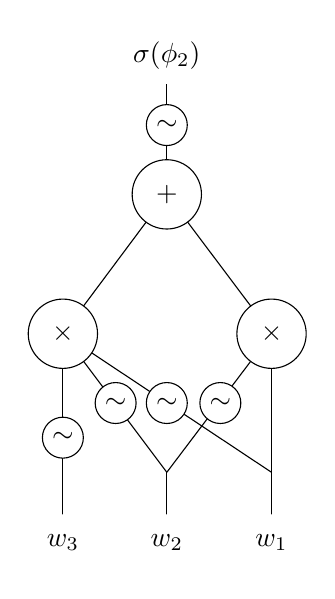
\begin{tikzpicture}
\definecolor{fillcolor}{RGB}{255,255,255}
\definecolor{highcolor}{RGB}{0,0,0}
\definecolor{lowcolor}{RGB}{0,0,0}
\definecolor{neutralcolor}{RGB}{0,0,0}
\definecolor{pathcolor}{RGB}{0,0,0}
\definecolor{background}{RGB}{225,225,225}
\draw (1.76,6.53) [thin,neutralcolor] -- (1.76,4.77);
\draw (1.76,4.77) [thin,neutralcolor] -- (0.44,3.00);
\draw (1.76,4.77) [thin,neutralcolor] -- (3.09,3.00);
\draw (0.44,3.00) [thin,neutralcolor] -- (3.09,1.24);
\draw (0.44,3.00) [thin,neutralcolor] -- (0.44,0.35);
\draw (0.44,3.00) [thin,neutralcolor] -- (1.76,1.24);
\draw (3.09,3.00) [thin,neutralcolor] -- (3.09,1.24);
\draw (3.09,3.00) [thin,neutralcolor] -- (1.76,1.24);
\draw (3.09,1.24) [thin,neutralcolor] -- (3.09,0.35);
\draw (1.76,1.24) [thin,neutralcolor] -- (1.76,0.35);
\draw [thin,fill=fillcolor,draw=fillcolor] (1.76,6.53) circle [radius=0.35];
\node at (1.76,6.53) {$\sigma(\phi_2)$};
\draw [thin,fill=fillcolor,draw=neutralcolor] (1.76,4.77) circle [radius=0.44];
\node at (1.76,4.77) {$+$};
\draw [thin,fill=fillcolor,draw=neutralcolor] (0.44,3.00) circle [radius=0.44];
\node at (0.44,3.00) {$\times$};
\draw [thin,fill=fillcolor,draw=neutralcolor] (3.09,3.00) circle [radius=0.44];
\node at (3.09,3.00) {$\times$};
\draw [thin,fill=neutralcolor,draw=neutralcolor] (3.09,1.24) circle [radius=0.00];
\node at (3.09,1.24) {};
\draw [thin,fill=neutralcolor,draw=neutralcolor] (1.76,1.24) circle [radius=0.00];
\node at (1.76,1.24) {};
\draw [thin,fill=fillcolor,draw=fillcolor] (3.09,0.35) circle [radius=0.35];
\node at (3.09,0.35) {$w_1$};
\draw [thin,fill=fillcolor,draw=fillcolor] (1.76,0.35) circle [radius=0.35];
\node at (1.76,0.35) {$w_2$};
\draw [thin,fill=fillcolor,draw=fillcolor] (0.44,0.35) circle [radius=0.35];
\node at (0.44,0.35) {$w_3$};
\draw [thin,fill=fillcolor,draw=neutralcolor] (1.76,5.65) circle [radius=0.26];
\node at (1.76,5.65) {$\sim$};
\draw [thin,fill=fillcolor,draw=neutralcolor] (1.76,2.12) circle [radius=0.26];
\node at (1.76,2.12) {$\sim$};
\draw [thin,fill=fillcolor,draw=neutralcolor] (1.11,2.12) circle [radius=0.26];
\node at (1.11,2.12) {$\sim$};
\draw [thin,fill=fillcolor,draw=neutralcolor] (2.44,2.12) circle [radius=0.26];
\node at (2.44,2.12) {$\sim$};
\draw [thin,fill=fillcolor,draw=neutralcolor] (0.44,1.68) circle [radius=0.26];
\node at (0.44,1.68) {$\sim$};
\end{tikzpicture}%%
}
    \end{minipage}
  }
  \caption{Schema \#2A for Formula $\phi_2 = (x_1 \lor x_2 \lor x_3) \land (\obar{x}_1 \lor x_2)$ and its Cost Computation}
\label{fig:p2-bdd:schema}
\end{figure}


\begin{figure}
  A).  CRAT File Contents
  \begin{center}
  \begin{tabular}{lcllll}
    \multicolumn{4}{c}{Proof line} & & \multicolumn{1}{c}{Explanation} \\
\midrule

    \makebox[5mm][l]{\tt 1} & \makebox[7mm]{\tt i}   & \makebox[20mm][l]{\tt 1 2 3 0}   &  \makebox[30mm]{}          & \makebox[5mm]{} & \makebox[40mm][l]{Input clause $C_1$}\\
    {\tt 2} & {\tt i}   & {\tt -1 2 0}  &            & & Input clause $C_2$ \\
    {\tt 3} & {\tt p}   & {\tt 4 -2 -3}  &            & & Declare $p_4 = \obar{x}_2 \pand \obar{x}_3$ \\
    {\tt 6} & {\tt p}   & {\tt 5 -1 4}  &             & & Declare $p_5 = \obar{x}_1 \pand p_4 = \obar{x}_1 \pand \obar{x}_2 \pand \obar{x}_3$ \\
    {\tt 9} & {\tt a}  & {\tt -5 0} & {\tt 7 8 5 4 1 0} & & Assert $t_1 = \obar{p}_5 = x_1 \lor x_2 \lor x_3$ \\
            & {\tt dc}  & {\tt 1 } & {\tt 3 6 9 0} & & Delete clause $C_1$\\
    {\tt 10} & {\tt p}   & {\tt 6 1 -2} &              & & Declare $p_6 = x_1 \pand \obar{x}_2$ \\    
    {\tt 13} & {\tt a} & {\tt -6 0} & {\tt 12 11 2 0}  & & Assert $t_2 = \obar{p}_6 = \obar{x}_1 \lor x_2$ \\
            & {\tt dc}  & {\tt 2 } & {\tt 10 13 0} & & Delete clause $C_2$\\
    {\tt 14} & {\tt s}   & {\tt 7 5 6}   & {\tt 7 11 0}  & & Declare $s_7 = \obar{t}_1 \por \obar{t}_2$ \\
    {\tt 17} & {\tt a}  & {\tt -7 0}       & {\tt 9 13 14 0} & & Assert $t_3 = \obar{s}_7 = t_1 \land t_2$ \\
             & {\tt dc}  & {\tt 9}          & {\tt 15 17 0} & & Delete $t_1$\\
             & {\tt dc}  & {\tt 13}         & {\tt 16 17 0} & & Delete $t_2$\\
  \end{tabular}
  \end{center}  
B). Proof Clauses
  \begin{center}
  \begin{tabular}{lcllll}
    \multicolumn{4}{c}{Clause} & & \multicolumn{1}{c}{Explanation} \\
\midrule
    \makebox[5mm][l]{\tt 1} & \makebox[7mm]{}   & \makebox[20mm][l]{\tt 1 2 3 0}   &  \makebox[30mm]{}          & \makebox[5mm]{} & \makebox[40mm][l]{Input clause $C_1$}\\
    {\tt 2} &    & {\tt -1 2 0}  &            & & Input clause $C_2$ \\
    {\tt 3} &   & {\tt 4 2 3 0} &     & & Defining clauses for $p_4$ \\
    {\tt 4} &   & {\tt -4 -2 0} &     & & \\
    {\tt 5} &   & {\tt -4 -3 0} &     & & \\

    {\tt 6} &   & {\tt 5 1 -4 0} &    & & Defining clauses for $p_5$ \\
    {\tt 7} &   & {\tt -5 -1 0} &     & & \\
    {\tt 8} &   & {\tt -5 4 0} &      & & \\

    {\tt 9} &   & {\tt -5 0} & {\tt 7 8 5 4 1 0} & & Assert $t_1 = \obar{p}_5 = x_1 \lor x_2 \lor x_3$ \\
            & {\tt dc}  & {\tt 1 } & {\tt 3 6 9 0} & & Delete clause $C_1$\\

    {\tt 10} &   & {\tt 6 -1 2 0}  &    & & Defining clauses for $p_6$ \\ 
    {\tt 11} &   & {\tt -6 1 0}    &  & & \\
    {\tt 12} &   & {\tt -6 -2 0}    &  & & \\ 
    {\tt 13} &  & {\tt -6 0} & {\tt 12 11 2 0}  & & Assert $t_2 = \obar{p}_6 = \obar{x}_1 \lor x_2$ \\
            & {\tt dc}  & {\tt 2 } & {\tt 10 13 0} & & Delete clause $C_2$\\
             &          & {\tt -5 -6 0} & {\tt 7 11 0}  & & Mutual exclusion proof for $s_7$ \\
    {\tt 14} &   & {\tt -7 5 6 0}  &     & & Defining clauses for $s_7$ \\ 
    {\tt 15} &   & {\tt  7 -5 0}    &  &  \\  
    {\tt 16} &   & {\tt  7 -6 0}    &  & &  \\
    {\tt 17} &   & {\tt -7 0}       & {\tt 9 13 0} & & Assert $t_3 = \obar{s}_7 = t_1 \land t_2$ \\
             & {\tt dc}  & {\tt 9}          & {\tt 15 17 0} & & Delete $t_1$\\
             & {\tt dc}  & {\tt 13}         & {\tt 16 17 0} & & Delete $t_2$\\
  \end{tabular}
  \end{center}  
  \caption{CRAT file \#2A for formula $\phi_2 = (x_1 \lor x_2 \lor x_3) \land (\obar{x}_1 \lor x_2)$, and the resulting set of proof clauses}
  \label{fig:p2-bdd:crat}
\end{figure}

As a more complex example, consider the Boolean formula $\phi_2$ given
by the conjunction of clauses $C_1 = x_1 \lor x_2 \lor x_3$ and $C_2 =
\obar{x}_1 \lor x_2$.  With this example, we also demonstrate the use
of DeMorgan's Laws to provide a more compact encoding of the formula,
similar to the use of these laws when encoding ITE operations in
Table~\ref{tab:ite}.

Figure~\ref{fig:p2-bdd:schema} shows a schema representing the formula,
and Figure~\ref{fig:p2-bdd:crat} shows the associated CRAT file and proof clauses.  This
proof was generated via a bottom-up strategy, such as would be created
using BDDs.  It creates schematic representations of the input
clauses and then forms their conjunction.  In the proof, unit
clauses are generated for the representations of the input clauses,
and then the input clauses are deleted.  These intermediate unit
clauses are used to justify a unit clause for the final root, and then
they are deleted.

Using DeMorgan's Laws, $C_1$ can be written as 
$t_1 = \neg [\obar{x}_1\land \obar{x}_2\land \obar{x}_3]$, and this can be
expressed using $\pand$ operations $s_4$ and $s_5$, shown in
Figure~\ref{fig:p2-bdd:schema}A\@.  (Note that $t_1$ in this case is
logically equivalent to root $t_1$ in the schema of
Figure~\ref{fig:c3:schema}A, but the use of negation enables it to be
represented with two operations rather than four.)  Similarly, $C_2$
can be written as $t_2 = \neg [x_1\land \obar{x}_2]$, and this can be
represented by $\pand$ operation $p_6$.
Terms $t_1$ and $t_2$ are asserted as unit clauses on proof lines 9 and 13,
allowing the input clauses to be deleted.
The conjunction $t_1 \land t_2$
can be written as $t_3 = \neg[\obar{t_1} \lor \obar{t_2}]$, represented by $\por$ operation $s_7$.
Term $t_3$ is asserted as a unit clause on proof line 17.
Based on this, the unit clauses for terms $t_1$ and
$t_2$ can be deleted.  Term $t_3$ then becomes the unique root of the cost
computation shown in Figure~\ref{fig:p2-bdd:schema}B\@.

\subsection{Example 2B}

\begin{figure}
  \centering{
    \begin{minipage}{0.4\textwidth}
      A) Schema   \\[2ex]
    \centering{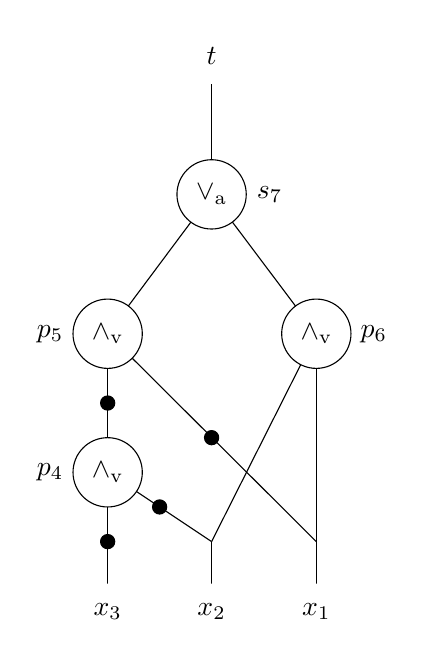
\begin{tikzpicture}
\definecolor{fillcolor}{RGB}{255,255,255}
\definecolor{highcolor}{RGB}{0,0,0}
\definecolor{lowcolor}{RGB}{0,0,0}
\definecolor{neutralcolor}{RGB}{0,0,0}
\definecolor{pathcolor}{RGB}{0,0,0}
\definecolor{background}{RGB}{225,225,225}
\draw (1.76,7.41) [thin,neutralcolor] -- (1.76,5.65);
\draw (1.76,5.65) [thin,neutralcolor] -- (0.44,3.88);
\draw (1.76,5.65) [thin,neutralcolor] -- (3.09,3.88);
\draw (0.44,3.88) [thin,neutralcolor] -- (3.09,1.24);
\draw [fill=neutralcolor,draw=neutralcolor] (1.76,2.56) circle [radius=0.09];
\draw (0.44,3.88) [thin,neutralcolor] -- (0.44,2.12);
\draw [fill=neutralcolor,draw=neutralcolor] (0.44,3.00) circle [radius=0.09];
\draw (3.09,3.88) [thin,neutralcolor] -- (3.09,1.24);
\draw (3.09,3.88) [thin,neutralcolor] -- (1.76,1.24);
\draw (3.09,1.24) [thin,neutralcolor] -- (3.09,0.35);
\draw (0.44,2.12) [thin,neutralcolor] -- (0.44,0.35);
\draw [fill=neutralcolor,draw=neutralcolor] (0.44,1.24) circle [radius=0.09];
\draw (0.44,2.12) [thin,neutralcolor] -- (1.76,1.24);
\draw [fill=neutralcolor,draw=neutralcolor] (1.10,1.68) circle [radius=0.09];
\draw (1.76,1.24) [thin,neutralcolor] -- (1.76,0.35);
\draw [thin,fill=fillcolor,draw=fillcolor] (1.76,7.41) circle [radius=0.35];
\node at (1.76,7.41) {$t$};
\draw [thin,fill=fillcolor,draw=neutralcolor] (1.76,5.65) circle [radius=0.44];
\node at (1.76,5.65) {$\lor_{\textrm{a}}$};
\draw [thin,fill=fillcolor,draw=neutralcolor] (0.44,3.88) circle [radius=0.44];
\node at (0.44,3.88) {$\land_{\textrm{v}}$};
\draw [thin,fill=fillcolor,draw=neutralcolor] (3.09,3.88) circle [radius=0.44];
\node at (3.09,3.88) {$\land_{\textrm{v}}$};
\draw [thin,fill=fillcolor,draw=neutralcolor] (0.44,2.12) circle [radius=0.44];
\node at (0.44,2.12) {$\land_{\textrm{v}}$};
\draw [thin,fill=neutralcolor,draw=neutralcolor] (3.09,1.24) circle [radius=0.00];
\node at (3.09,1.24) {};
\draw [thin,fill=neutralcolor,draw=neutralcolor] (1.76,1.24) circle [radius=0.00];
\node at (1.76,1.24) {};
\draw [thin,fill=fillcolor,draw=fillcolor] (3.09,0.35) circle [radius=0.35];
\node at (3.09,0.35) {$x_1$};
\draw [thin,fill=fillcolor,draw=fillcolor] (1.76,0.35) circle [radius=0.35];
\node at (1.76,0.35) {$x_2$};
\draw [thin,fill=fillcolor,draw=fillcolor] (0.44,0.35) circle [radius=0.35];
\node at (0.44,0.35) {$x_3$};
\node [right] at (2.21,5.65) {$s_7$};
\node [right] at (3.53,3.88) {$p_6$};
\node [left] at (0.00,3.88) {$p_5$};
\node [left] at (0.00,2.12) {$p_4$};
\end{tikzpicture}%%
}
    \end{minipage}
    \begin{minipage}{0.4\textwidth}
    B) Cost Computation\\[2ex]
    \centering{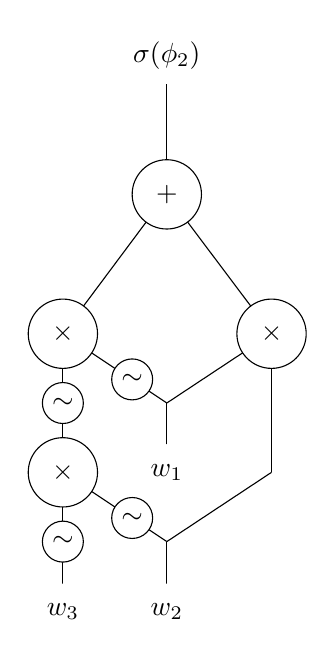
\begin{tikzpicture}
\definecolor{fillcolor}{RGB}{255,255,255}
\definecolor{highcolor}{RGB}{0,0,0}
\definecolor{lowcolor}{RGB}{0,0,0}
\definecolor{neutralcolor}{RGB}{0,0,0}
\definecolor{pathcolor}{RGB}{0,0,0}
\definecolor{background}{RGB}{225,225,225}
\draw (1.76,7.41) [thin,neutralcolor] -- (1.76,5.65);
\draw (1.76,5.65) [thin,neutralcolor] -- (0.44,3.88);
\draw (1.76,5.65) [thin,neutralcolor] -- (3.09,3.88);
\draw (0.44,3.88) [thin,neutralcolor] -- (1.76,3.00);
\draw (0.44,3.88) [thin,neutralcolor] -- (0.44,2.12);
\draw (3.09,3.88) [thin,neutralcolor] -- (1.76,3.00);
\draw (3.09,3.88) [thin,neutralcolor] -- (3.09,2.12);
\draw (1.76,3.00) [thin,neutralcolor] -- (1.76,2.12);
\draw (0.44,2.12) [thin,neutralcolor] -- (0.44,0.35);
\draw (0.44,2.12) [thin,neutralcolor] -- (1.76,1.24);
\draw (3.09,2.12) [thin,neutralcolor] -- (1.76,1.24);
\draw (1.76,1.24) [thin,neutralcolor] -- (1.76,0.35);
\draw [thin,fill=fillcolor,draw=fillcolor] (1.76,7.41) circle [radius=0.35];
\node at (1.76,7.41) {$\sigma(\phi_2)$};
\draw [thin,fill=fillcolor,draw=neutralcolor] (1.76,5.65) circle [radius=0.44];
\node at (1.76,5.65) {$+$};
\draw [thin,fill=fillcolor,draw=neutralcolor] (0.44,3.88) circle [radius=0.44];
\node at (0.44,3.88) {$\times$};
\draw [thin,fill=fillcolor,draw=neutralcolor] (3.09,3.88) circle [radius=0.44];
\node at (3.09,3.88) {$\times$};
\draw [thin,fill=fillcolor,draw=neutralcolor] (0.44,2.12) circle [radius=0.44];
\node at (0.44,2.12) {$\times$};
\draw [thin,fill=neutralcolor,draw=neutralcolor] (1.76,3.00) circle [radius=0.00];
\node at (1.76,3.00) {};
\draw [thin,fill=neutralcolor,draw=neutralcolor] (1.76,1.24) circle [radius=0.00];
\node at (1.76,1.24) {};
\draw [thin,fill=neutralcolor,draw=neutralcolor] (3.09,2.12) circle [radius=0.00];
\node at (3.09,2.12) {};
\draw [thin,fill=fillcolor,draw=fillcolor] (1.76,2.12) circle [radius=0.35];
\node at (1.76,2.12) {$w_1$};
\draw [thin,fill=fillcolor,draw=fillcolor] (1.76,0.35) circle [radius=0.35];
\node at (1.76,0.35) {$w_2$};
\draw [thin,fill=fillcolor,draw=fillcolor] (0.44,0.35) circle [radius=0.35];
\node at (0.44,0.35) {$w_3$};
\draw [thin,fill=fillcolor,draw=neutralcolor] (1.32,3.30) circle [radius=0.26];
\node at (1.32,3.30) {$\sim$};
\draw [thin,fill=fillcolor,draw=neutralcolor] (0.44,3.00) circle [radius=0.26];
\node at (0.44,3.00) {$\sim$};
\draw [thin,fill=fillcolor,draw=neutralcolor] (1.32,1.54) circle [radius=0.26];
\node at (1.32,1.54) {$\sim$};
\draw [thin,fill=fillcolor,draw=neutralcolor] (0.44,1.24) circle [radius=0.26];
\node at (0.44,1.24) {$\sim$};
\end{tikzpicture}%%
}
    \end{minipage}
  }
\caption{Schema \#2B for Formula $\phi_2 = (x_1 \lor x_2 \lor x_3) \land (\obar{x}_1 \lor x_2)$ and its Cost Computation}
\label{fig:p2-cdcl:schema}
\end{figure}


\begin{figure}
  A).  CRAT File Contents
  \begin{center}
  \begin{tabular}{llllll}
    \multicolumn{4}{c}{File line} & & \multicolumn{1}{c}{Explanation} \\
\midrule
    \makebox[5mm][l]{\tt 1} & \makebox[7mm]{}   & \makebox[20mm][l]{\tt 1 2 3 0}   &  \makebox[30mm]{}          & \makebox[5mm]{} & \makebox[40mm][l]{Input clause $C_1$}\\
            {\tt 2} & {\tt i}   & {\tt -1 2 0}  &            & & Input clause $C_2$ \\
            {\tt 3} & {\tt p}   & {\tt 4 -2 -3}  &            & & Declare $p_4 = \obar{x}_2 \pand \obar{x}_3$ \\
    {\tt 6} & {\tt p}   & {\tt 5 -1 -4}  &             & & Declare $p_5 = \obar{x}_1 \pand \obar{p}_4$ \\
    {\tt 9} & {\tt p}   & {\tt 6 1 2} &              & & Declare $p_6 = x_1 \pand x_2$ \\    
    {\tt 12} & {\tt s}   & {\tt 7 5 6}   & {\tt 7 10 0}  & & Declare $s_7 = p_5 \por p_6$ \\
    {\tt 15} & {\tt a}  & {\tt 1 -4 0}    & {\tt 4 5 1 0} & & Justify $\obar{x}_1 \rightarrow \obar{p}_4$ \\
    {\tt 16} & {\tt a}  & {\tt 1 7 0}     & {\tt 13 6 15 0} & & Justify $\obar{x}_1 \rightarrow s_7$ \\
    {\tt 17} & {\tt a}  & {\tt -1 7 0}    & {\tt 14 9 2 0} & & Justify $x_1 \rightarrow s_7$ \\
    {\tt 18} & {\tt a}  & {\tt 7 0}       & {\tt 16 17 0}  & & Justify unit clause $t = s_7$ \\
             & {\tt dc}  & {\tt 1}         & {\tt 3 8 10 12 18 0} & & Delete $C_1$\\
             & {\tt dc}  & {\tt 2}         & {\tt 11 7 12 18 0} & & Delete $C_2$\\
  \end{tabular}
  \end{center}  
B). Proof Clauses
  \begin{center}
  \begin{tabular}{llllll}
    \multicolumn{4}{c}{File line} & & \multicolumn{1}{c}{Explanation} \\
\midrule
    \makebox[5mm][l]{\tt 1} & \makebox[7mm]{}   & \makebox[20mm][l]{\tt 1 2 3 0}   &  \makebox[30mm]{}          & \makebox[5mm]{} & \makebox[40mm][l]{Input clause $C_1$}\\
    {\tt 2} &    & {\tt -1 2 0}  &            & & Input clause $C_2$ \\
    {\tt 3} &   & {\tt 4 2 3 0} &     & & Defining clauses for $p_4$ \\
    {\tt 4} &   & {\tt -4 -2 0} &     & & \\
    {\tt 5} &   & {\tt -4 -3 0} &     & & \\
    {\tt 6} &   & {\tt 5 1 4 0} &     & & Defining clauses for $p_5$ \\
    {\tt 7} &   & {\tt -5 -1 0} &     & & \\
    {\tt 8} &   & {\tt -5 -4 0} &     & & \\
    {\tt 9} &   & {\tt 6 -1 -2 0}&     & & Defining clauses for $p_6$ \\ 
    {\tt 10} &   & {\tt -6 1 0}    &  & & \\
    {\tt 11} &   & {\tt -6 2 0}    &  & & \\ 
     &           & {\tt -5 -6}   & {\tt 7 10 0}  & & Mutual exclusion proof for $s_7$ \\
    {\tt 12} &   & {\tt -7 5 6 0}  &     & & Defining clauses for $s_7$ \\ 
    {\tt 13} &   & {\tt  7 -5 0}    &  & & \\  
    {\tt 14} &   & {\tt  7 -6 0}    &  & & \\
    {\tt 15} &   & {\tt 1 -4 0}    & {\tt 4 5 1 0} & & Justify $\obar{x}_1 \rightarrow \obar{p}_4$ \\
    {\tt 16} &   & {\tt 1 7 0}     & {\tt 13 6 15 0} & & Justify $\obar{x}_1 \rightarrow s_7$ \\
    {\tt 17} &   & {\tt -1 7 0}    & {\tt 14 9 2 0} & & Justify $x_1 \rightarrow s_7$ \\
    {\tt 18} &   & {\tt 7 0}       & {\tt 16 17 0}  & & Justify unit clause $t = s_7$ \\
             & {\tt dc}  & {\tt 1}         & {\tt 3 15 0} & & Delete $C_1$\\
             & {\tt dc}  & {\tt 2}         & {\tt 11 7 12 18 0} & & Delete $C_2$\\
  \end{tabular}
  \end{center}  
  \caption{CRAT file \#2B for formula $\phi_2 = (x_1 \lor x_2 \lor x_3) \land (\obar{x}_1 \lor x_2)$, and the resulting set of proof clauses}
  \label{fig:p2-cdcl:crat}
\end{figure}

Figure~\ref{fig:p2-cdcl:schema} shows an alternate schema representing
the same formula $\phi_2$ as in Example~2A, and
Figure~\ref{fig:p2-cdcl:crat} shows the associated CRAT proof.  This
proof was generated via a top-down strategy, such as would be created
using a model counter based on CDCL\@.  It starts by splitting on
variable $x_1$.  Clause $C_1$ is trivially satisfied when $x_1$ is
assigned $\tautology$, and clause $C_2$ becomes the clause $C'_2 =
x_2$.  On the other hand, clause $C_2$ is trivially satisfied when
$x_1$ is assigned $\nil$, and clause $C_1$ becomes $C'_1 = x_2 \lor
x_3$.  Clause $C'_1$ can be represented schematically as
$\neg[\obar{x}_2 \pand \obar{x}_3]$, with this operation labeled $p_4$
in Figure~\ref{fig:p2-cdcl:schema}A\@.  The splitting on variable
$x_1$ can be rejoined as $\ite(x_1, x_2, \obar{p}_4)$, and this ITE
operation can be expressed using the product operations $p_5$ and
$p_6$, joined by the sum operation $t = s_7$.

The two schemas shown in Figures~\ref{fig:p2-bdd:schema}A and
\ref{fig:p2-cdcl:schema}A have similar structure.  They have very
different negation patterns, but they are logically equivalent.  Their
associated cost computations (Figures~\ref{fig:p2-bdd:schema}B and
\ref{fig:p2-cdcl:schema}B) also yield the same results for arbitrary
weights $w_1$, $w_2$, and $w_3$.

The CRAT proof for the top-down approach follows a different pattern than does the proof based on a bottom-up construction.
It does
not create any intermediate unit clauses.  Instead, it constructs a proof
that the root $t = s_7$ holds as a unit clause by splitting into the
two assignments for variable $x_1$.  The proof that
$\obar{x}_1 \rightarrow s_7$ (proof line 16) builds on the proof that
$\obar{x}_1 \rightarrow \obar{p}_4$ (proof line 15), which derives from clause $C_1$.
The proof that $x_1 \rightarrow x_7$ (proof line 17) derives from clause $C_2$.
These two are combined to yield the unit clause $s_7$ (proof line 18).
Given this unit clause, the two input clauses can then be deleted.


\section{Looking Ahead}

\subsection{Implementing Certified Counters}

Given an arbitrary CNF formula, we can use BDD operations to generate
a schematic representation.  The proof generation can follow the
methods we have used for generating unsatisfiability proofs of Boolean
formulas~\cite{bryant:tacas:2021} and dual proofs of quantified
Boolean formulas~\cite{bryant:cade:2021}.
Each BDD node can be expressed as an ITE operation and
make use of the encodings shown in Table~\ref{tab:ite}.

A second class of model counters proceeds top-down, based on the CDCL
framework.  These choose a splitting variable $x$ and recursively
construct schemas $S_1$ and $S_0$ for the two assignments to the
variable.  These are combined as $\ite(x, S_1, S_0)$, using one of the
encodings of $\ite$ shown in Table~\ref{tab:ite}.  Like CDCL, the
top-down algorithm can make use of unit propagation, conflict
detection, and clause learning.  It can also make use of {\em
  variable} partitioning.  That is, suppose for some partial
assignment to the variables, the input clauses decompose into two or
more sets over disjoint variables.  Then the schema for each of these
partitions can be generated separately, and these are joined via the $\pand$
operation.

%% \subsection{Tseitin Variable Optimization}

%% Many problems cannot be directly encoded in CNF without an exponential
%% blowup.  This can be avoided by introducing auxilliary variables.  A
%% particular approach to these encodings makes use of {\em Tseitin}
%% variables.  The general scheme with these is to let a variable $z$
%% encode a subformula $F$ over input and prior Tseitin variables by
%% adding clauses encoding $z \leftrightarrow F$.  A particular property
%% of this encoding is that if we let ${\cal C}_z$ (respectively ${\cal
%%   C}_{\obar{z}}$) denote the clauses in which literal $z$ (resp.,
%% $\obar{z}$) occcurs

\subsection{TO-DO List}

\begin{itemize}
\item Proof Framework
  \begin{itemize}
  \item Generalities and details of the format
  \item Can some form of abstraction be incorporated?
    \begin{itemize}
    \item Want to abstract a subformula to consider only on its cost and dependency set
    \item Could represent with fresh extension variable
    \item But how to prove logical equivalence?
    \end{itemize}
  \end{itemize}

\item Checker
  \begin{itemize}
  \item Working prototype
  \item C/C++ (or Rust?)
  \item Formally verified
  \end{itemize}

\item Counters
\begin{itemize}
\item BDD-based
  \begin{itemize}
  \item Prototype
  \item C/C++
  \end{itemize}

  \item SDD-based
  \begin{itemize}
  \item Bottom-up
  \item Top-down
  \end{itemize}

\item Others?
\end{itemize}
\end{itemize}


\bibliography{references}


\end{document}


